Damit ihr nicht ganz verloren im gro\ss en Uni-Wirrwarr umher irrt und
  nicht immer das Gefühl haben müsst, etwas sehr Wichtiges geht
  voll an euch vorbei, findet ihr hier eine Übersicht über die wichtigsten Begriffe:

\begin{description}

%\item [Schwerpunkt-/Nebenfach:] Wenn ihr reine Informatik studiert, benötigt ihr ein Schwerpunktfach, also ein zweites Fach in dem ihr 18 LP erwerben müsst. Bei der Führung über den Sand werden Schwerpunktfächer vorgestellt, später wird die Fachschaft noch eine Info-Veranstaltung speziell zum Schwerpunktfach anbieten. 

\item [Schwerpunkt-/Nebenfach:] Wenn ihr reine Informatik studiert, steht es
  euch offen, ob ihr 18 ECTS in ein Schwerpunktfach oder in ÜbK
  investieren wollt. Letzteres ermöglicht euch eine freiere Wahl an Kursen.

\item [Übungen:] Zu den meisten Veranstaltungen des Fachbereichs werden neben den Vorlesungen noch Übungen angeboten, welche euch helfen, den gelernten Stoff zu verinnerlichen. Meist könnt ihr über die Übungsblätter, die ihr wöchentlich oder zweiwöchentlich abgeben könnt, einen Bonus für eure Klausurnote erarbeiten. In machen Vorlesungen kann aber auch eine Mindestpunktzahl in den Übungen Voraussetzung für die Klausur sein.

Da die dazu zu lösenden Aufgaben manchmal recht heftig und zeitaufwändig ausfallen, empfiehlt es sich:

\begin{itemize}

\item \textbf{sofort voll einzusteigen}, denn die Aufgaben werden von Mal
  zu Mal schwerer.

\item sich eine \textbf{Arbeitsgruppe} zu suchen, denn alleine ist man
  als "`Normalbegabter"' fast verloren. Meistens darf eine
  Arbeitsgruppe (2-3 Studis) sogar eine gemeinsame Lösung abgeben!

\item auch dann Übungen zu machen, wenn es keine Pflichtaufgaben sind --
  die Klausur kommt bestimmt.

\end {itemize}

\begin{center}
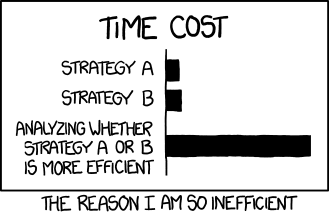
\includegraphics[width=0.5\hsize]{shared/xkcd/efficiency.png}
\end{center}


(Don't panic -- Die Matheübungszettel sind zu Anfang zwar der gro\ss e
  Schocker, die Prüfungen laufen aber in gemä\ss igterem Rahmen ab.)

\item [Vorlesungsverzeichnis:] Eine Übersicht über alle Veranstaltungen der Universität findet ihr seit dem April 2020 auf ALMA\footnote{\link{https://alma.uni-tuebingen.de}{ALMA}}. Dort findet ihr auch später eine Übersicht über eure Noten und könnt euch Studienbescheinigungen runterladen.
Außerdem finden hier die Anmeldungen zu den Klausuren statt.
 
\item [Eduroam:] Eduroam ist ein weltweiter Verbund von Bildungseinrichtungen, welcher es ermöglicht, an allen teilnehmenden Bildungseinrichtungen mit ein und der selben Kennung ins Internet zu gehen.
Eine Anleitung, wie man Eduroam richtig einrichtet findet ihr im Infrastruktur-Kapitel.

\item [ZDV:] Das Zentrum für Datenverarbeitung (ZDV) ist das Rechenzentrum der Universität und betreut die zahlreichen Rechner und Server, welche auch von Studierenden genutzt werden können. Vom ZDV solltet ihr nach eurer Immatrikulation auch ein Schreiben mit eurem ZDV Benutzernamen und einem Passwort bekommen haben. Diese ermöglichen euch die Nutzung der Uni-Infrastruktur.

\item [Computer Pool:] CIP Pools sind von der Universität betriebene Räume in denen Rechner des ZDVs stehen, die man als Studierender mit seiner ZDV Kennung nutzen kann.

\item[BAföG:] Das Bundesausbildungsförderungsgesetz unterstützt Studierende und Auszubildende aus einkommensschwachen Elternhäusern. Ob und wie ihr BAföG bekommt könnt ihr hier nachschauen: \url{https://www.bafoeg-rechner.de/}	%TODO insert \link{}{}?

\item[Mensa:] Die Mensen sind der Ort in dem man sich zum (un-)regelmäßigen Mittagessen trifft. Jede Mensa hat einen Speiseplan, welchen man auf der Seite des Studierendenwerks oder in der \emph{my-stuwe}-App einsehen kann\footnote{\url{https://www.my-stuwe.de/mensa/}}.	%TODO insert \link{}{}?

\vfill

\begin{center}
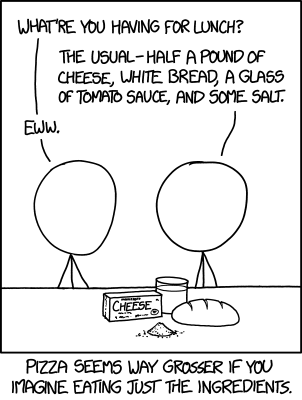
\includegraphics[width=0.35\hsize]{shared/xkcd/lunch.png}
\end{center}

\pagebreak

\end{description}
